%%%% fs-run-time-data-flow  FlameStream data flow

\label {fs-data-flow}

{\bf TODO:} preabe
Сейчас опишем тратата потом труту.
Барьер отпиливаем. 
Оставшиеся вопросы в оптимистик коллижен манагемент.

\subsection{Data flow}

The top level of our data flow abstraction is a {\it stream}. Stream is represented by an ordered unlimited sequence of data items. Data item is a {\it payload} and a {\it meta-data} associated with it. 

\[DataItem := (Payload, Meta)\]

Payload is an arbitrary user-provided data. Meta-data is a structured system-assigned information. The primary purpose of the meta-data is to impose the total order on data items. 

Data payloads are got in stream through {\it front} and got out through {\it barrier}. Particularly, front creates data items from input payloads by assigning them meta-data. Inside stream, data items can be dropped or their payloads and metas can be transformed. Eventually, barrier removes meta-information and outputs back pure payloads. High level view of our stream is shown on the figure~\ref{stream}.

\begin{figure}[htbp]
  \centering
  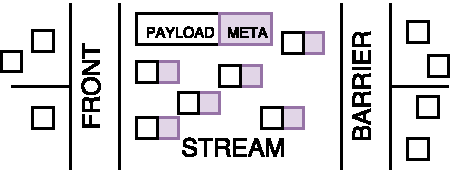
\includegraphics[width=0.48\textwidth]{pics/stream}
  \caption{Data flow}
  \label {stream}
\end{figure}

\subsection{Computaion flow}

The stream between front and barrier is handled by a directed data flow graph. Each node of the graph represents single operation, which can have multiple inputs and outputs. Edges indicate the order of these operations. Data items are processed one-by-one in a "streaming" manner. The figure~\ref{logical-graph-figure} shows the example of data flow graph.

Our model allows cycles in the graph while data flow graphs are commonly assumed to be acyclic (DAGs) 
~\cite{Zaharia:2016:ASU:3013530.2934664, Carbone:2017:SMA:3137765.3137777}. Moreover, as we show further, there are cases when cycles are required, e.g. for MapReduce-based algorithms. 

\subsection{Physical deployment and partitioning}
Data flow graph is distributed among computation unit. Each computational unit in our runtime runs process called {\it worker}, and each worker executes complete data flow graph. Every worker is assigned by an integer interval. Intervals are not intersected and cover the range of 32-bit signed integer.

Each input of a operation is assigned by user-provided hash function called {\it balancing function}. This function is applied to the payload of data items and determines partitioning. Data items are repartitioned before each operation. After that, corresponding data item is sent to the worker, which is responsible for the computed value. Therefore, load balancing explicitly depends on the balancing functions of the operations. The balancing functions are the part of business logic, because optimal balancing requires the knowledge of payload distribution. Possible partitioning of this graph on two nodes is shown on the figure~\ref{physical-graph-figure}.

\begin{figure}[htbp]
  \centering
  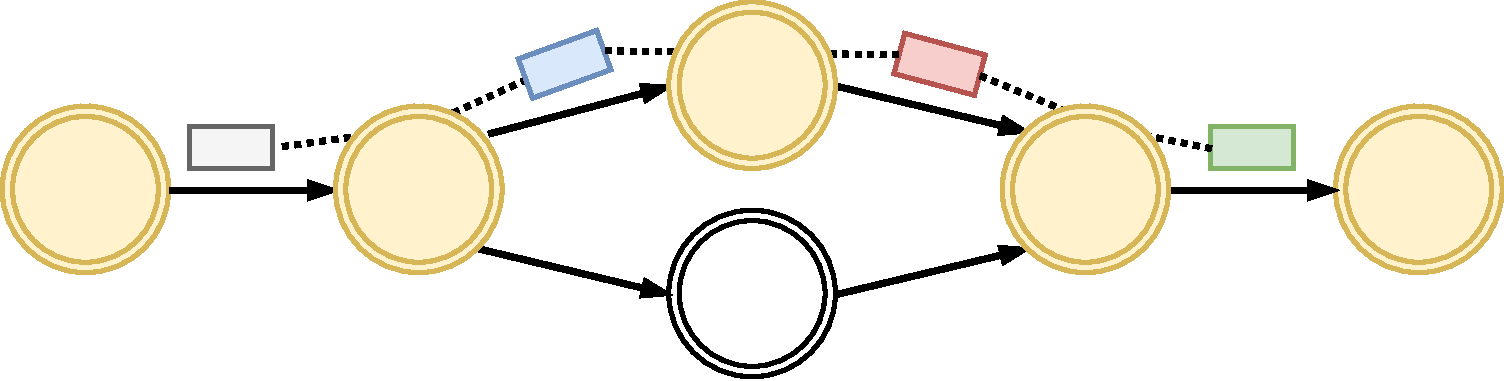
\includegraphics[width=0.48\textwidth]{pics/logical-graph}
  \caption{An example of the data flow graph}
  \label {logical-graph-figure}
\end{figure}

\begin{figure}[htbp]
  \centering
  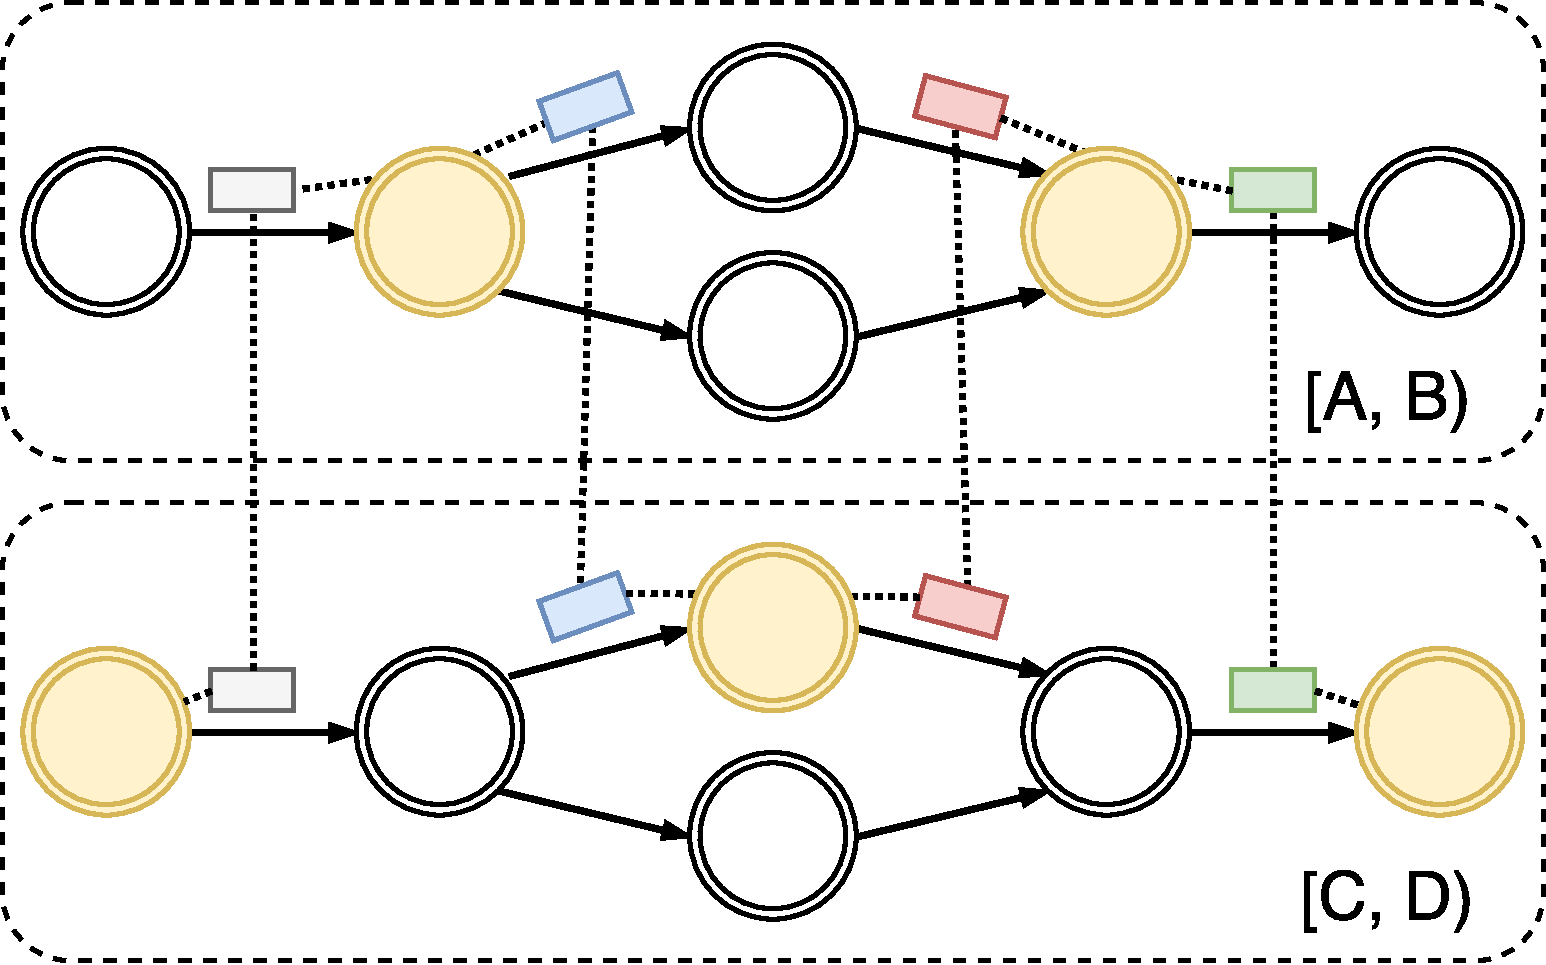
\includegraphics[width=0.48\textwidth]{pics/physical-graph}
  \caption{Possible partitioning of the data flow graph}
  \label {physical-graph-figure}
\end{figure}

\subsection{Ordering model}

As it was mentioned above, meta-information imposes an explicit total order on data items. Without diving into the details, it should be noted that the order of items is maintained across different fronts.

Let {\it image} be an output data item of an operation and {\it preimage} is a corresponding input item. In this terms, the order of images is preserved, i.e. the order of images is the same as the order of preimages. Moreover, the image of the item follows its preimage but precedes the next item. The concept of ordering is shown on the figure <>.

We assume that input items of the operations are strictly ordered. After the meta-data is assigned to data item at the front, the rest of computations become deterministic.

\subsection{Operations}

The set of available operations is limited by the following list.

{\bf Map} applies user-defined function to the payload of an input item. This function returns a sequence of data items with new payloads.

{\bf Broadcast} replicates an input item to the specified number of operations or sinks. 

{\bf Merge} operation is initialized with specified number of input nodes. Each input item from all inputs copied to the single output.

{\bf Grouping} has a {\it window size} parameter. Grouping stores input items in distinct buckets by the value of the input balancing function applied to payload. When the next item arrives to the grouping, it is appended to the corresponding bucket. Each time item grouping outputs window-sized {\it tuple item}, which consists of the last items of this bucket. The data items within tuple are ordered by the meta-information. If the size of bucket is less than window, all items of the bucket are taken. Grouping is the only operation that maintains state. To prevent collisions user can define equivalence relation to ensure that items with distinct payloads are got in the distinct buckets.

The following example illustrates the semantics of the operation. The grouping accepts items with payload represented as natural numbers: 1,2,3, etc. The hash function returns 1 if the number is even and 0 otherwise. If the window is set to 3, the output is:

\[(1), (2), (1|3), (2|4), (1|3|5), (2|4|6), (3|5|7), (4|6|8)...\]

The important property of the grouping is that the result is uniquely determined by the last element in the tuple. Therefore, grouping is the bijective mapping. Additionally, the results among items with different values of hash function are independent.

\subsection{User-defined parameters}

User is able to set up the following parameters:

\begin{enumerate}
  \item{Computation flow}
  \item{Balancing functions of the inputs}
  \item{Map functions}
  \item{Grouping windows}
\end{enumerate}

This parameters can produce more than one graph, which can yield equivalent results. Choosing among them is a performance optimization problem.    

It is important to mention, that there are no parameters for state-management. Therefore, business-logic is stateless. Nevertheless, the operations set is enough to implement any MapReduce transformation.
